\chapter{Evaluation}
In questo capitolo verranno riportati e valutati i risultati ottenuti dall’intero processo KDD.

\section{Valutazione dei risultati}

Il processo KDD terminerà con successo se si riuscirà a costruire il miglior modello di predizione in termini di maggior copertura di istanze rispetto agli algoritmi standard, ottenuto confrontando varie tecniche di modellazione.

\subsection{KnowledgeFlow}

\begin{figure}[hbtp!]
	\centering
	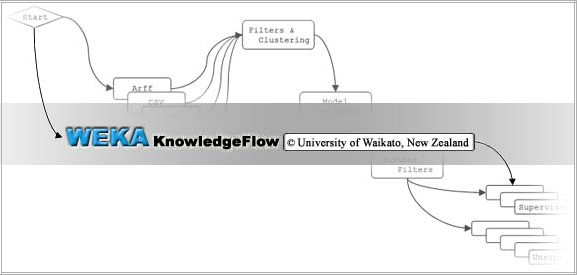
\includegraphics[width=0.6\textwidth]{./images/kf}
  	\caption{Logo di Weka KnowledgeFlow}  
\end{figure}

Per velocizzare le operazioni di confronto tra diverse tecniche di modeling si è scelto di usare lo strumento \textbf{KnowledgeFlow}, fornito sempre da Weka.

In KnowledgeFlow, l'utente può selezionare le componenti di Weka dalla barra degli strumenti, trascinarle su un canvas e collegarle l'una all'altra per formare un flusso per elaborare ed analizzare dati. Sono disponibili molti filtri, classificatori ed altri algoritmi già disponibili nell'Explorer di Weka, insieme ad altri strumenti, tipo la possibilità di salvare i risultati dell'elaborazione su un file, vedere grafici ecc.
 

Caratteristiche di KnowledgeFlow:
\begin{itemize}
	\item Layout intuitivo per rappresentare il flusso dei dati.
	\item Elaborazione dei dati in modalità batch o incrementale
    \item Elaborazione di più batch o stream in parallelo (ogni flusso ha il suo thread dedicato).
    \item Concatenazione di filtri.
    \item Visualizzazione delle performance dei classificatori al termine dell'elaborazione.
\end{itemize}

\subsection{Configurazioni}

Le varie configurazioni hanno previsto l'utilizzo di 3 tecniche di modeling, \textbf{IB1}, \textbf{Naive Bayes} e \textbf{C4.5} (quest'ultima implementata con l'algortimo J48). Ognuna ha lavorato sul dataset completo con tutti gli attributi iniziali e sulla sua versione ridotta ottenuta dalla feature selection. Inoltre per IB1 sono stati considerati diversi livelli di \emph{neighbours}, ovvero 1, 3 e 5.

Questo è lo schema del workflow senza feature selection:

\begin{figure}[hbtp!]
	\hspace*{-1.1in}
	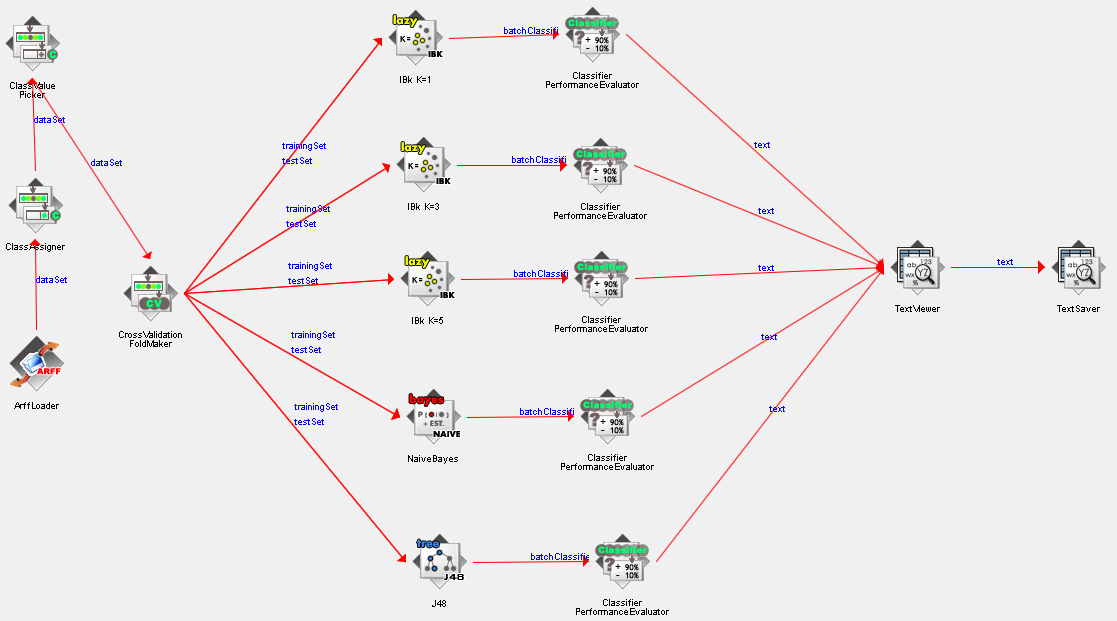
\includegraphics[width=1.4\textwidth]{./images/flow_no_featsel}
\end{figure}

Questo invece è lo schema con feature selection; l'unica differenza è la presenza della componente di filtraggio "AttributeSelection":

\begin{figure}[hbtp!]
	\hspace*{-1.1in}
	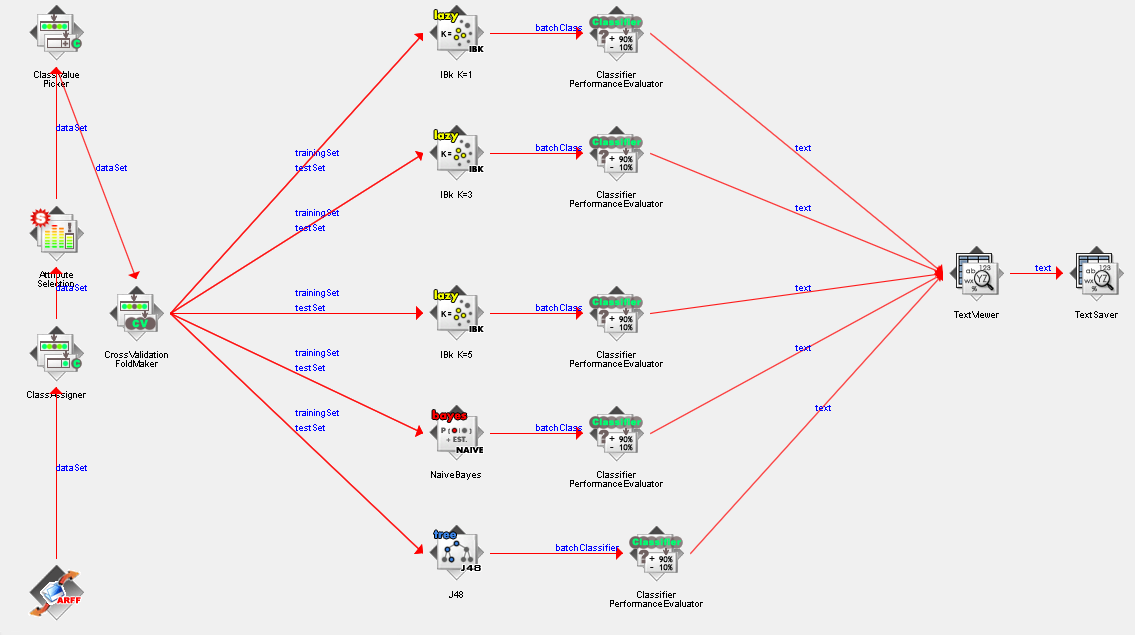
\includegraphics[width=1.4\textwidth]{./images/flow_featsel}
\end{figure}

% \begin{sidewaysfigure}
% 	\centering
% 	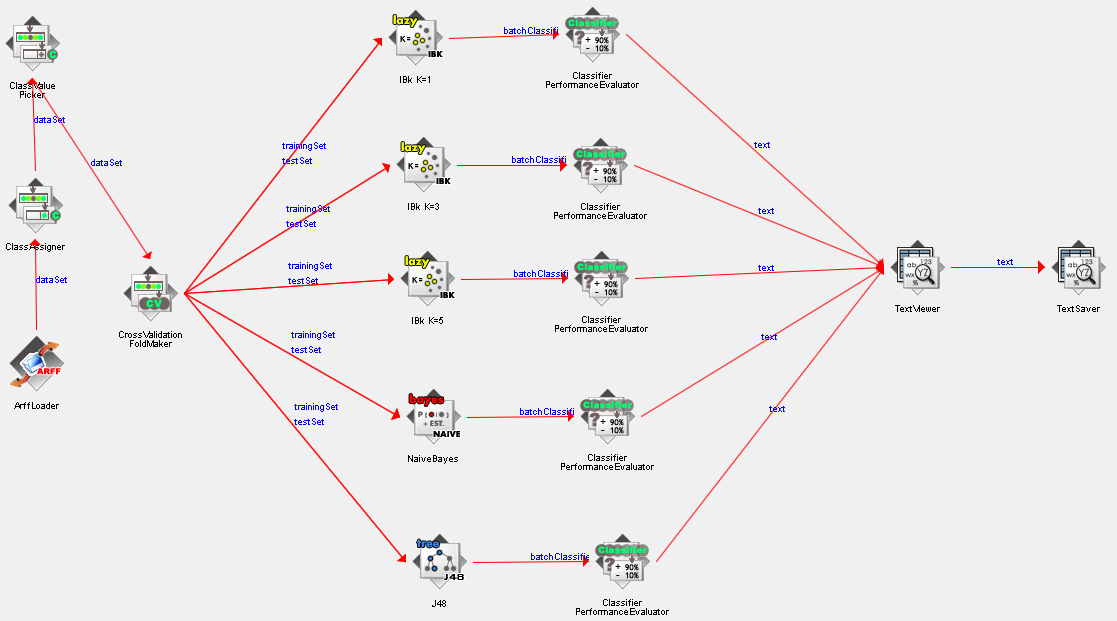
\includegraphics[width=1\textwidth]{./images/flow_no_featsel}
% \end{sidewaysfigure}

% Questo invece è lo schema con feature selection; l'unica differenza è la presenza della componente di filtraggio "AttributeSelection":

% \begin{sidewaysfigure}
% 	\centering
% 	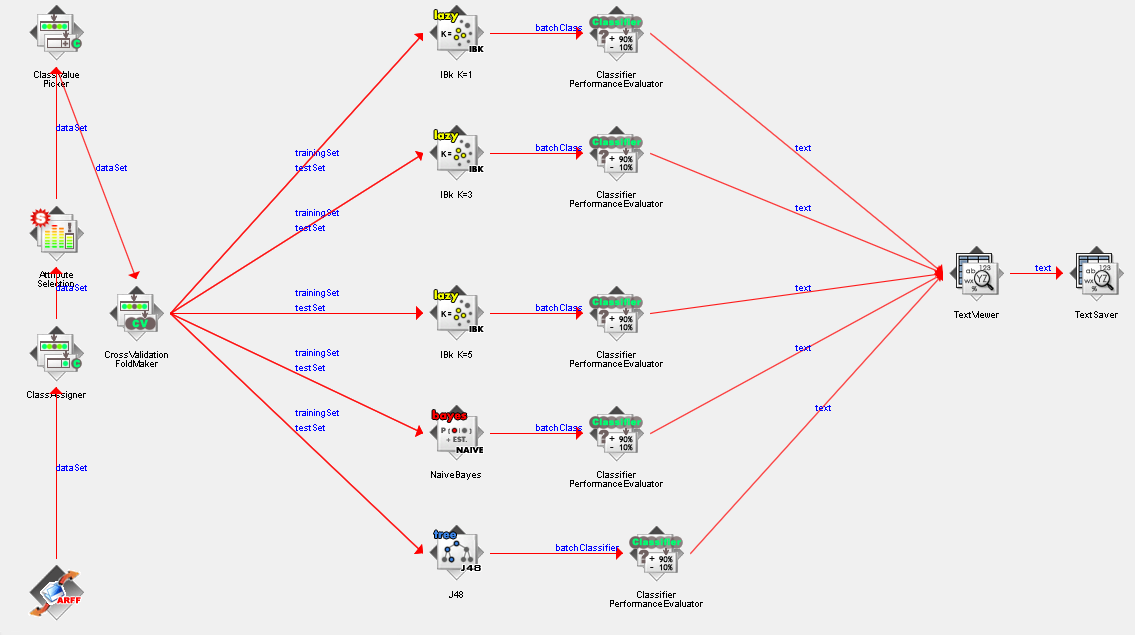
\includegraphics[width=1\textwidth]{./images/flow_featsel}
% \end{sidewaysfigure}

\subsection{Risultati delle configurazioni}
In questa sezione verranno elencati i risultati dell'esecuzione di KnowledgeFlow in base alle diverse configurazioni. \newline

La prima macro-configurazione ha previsto l'esecuzione \textbf{senza Feature selection}: \newline

\raggedright
\textbf{\Large Naive Bayes}

\begin{verbatim}
=== Evaluation result ===

Scheme: NaiveBayes
Relation: cup98LRN


Correctly Classified Instances        5617               58.8722 %
Incorrectly Classified Instances      3924               41.1278 %
Kappa statistic                          0.1776
Mean absolute error                      0.4123
Root mean squared error                  0.6133
Relative absolute error                 82.4696 %
Root relative squared error            122.6573 %
Coverage of cases (0.95 level)          68.9655 %
Mean rel. region size (0.95 level)      60.6435 %
Total Number of Instances             9541     

=== Detailed Accuracy By Class ===

           TP Rate  FP Rate  Precision  Recall   F-Measure  ROC Area  Class
           0,683    0,505    0,574      0,683    0,624      0,620     1
           0,495    0,317    0,610      0,495    0,546      0,620     0
W. Avg.    0,589    0,411    0,592      0,589    0,585      0,620          

=== Confusion Matrix ===

    a    b   <-- classified as
 3255 1511 |    a = 1
 2413 2362 |    b = 0
\end{verbatim}

\textbf{\Large C4.5 (J48)}

\begin{verbatim}
=== Evaluation result ===

Scheme: J48
Options: -C 0.25 -M 2
Relation: cup98LRN


Correctly Classified Instances        4833               50.6551 %
Incorrectly Classified Instances      4708               49.3449 %
Kappa statistic                          0.0132
Mean absolute error                      0.4999
Root mean squared error                  0.5001
Relative absolute error                 99.9836 %
Root relative squared error            100.0117 %
Coverage of cases (0.95 level)          99.9895 %
Mean rel. region size (0.95 level)      99.9843 %
Total Number of Instances             9541     

=== Detailed Accuracy By Class ===

           TP Rate  FP Rate  Precision  Recall   F-Measure  ROC Area  Class
           0,538    0,525    0,506      0,538    0,521      0,506     1
           0,475    0,462    0,507      0,475    0,491      0,506     0
W. Avg.    0,507    0,493    0,507      0,507    0,506      0,506      

=== Confusion Matrix ===

    a    b   <-- classified as
 2565 2201 |    a = 1
 2507 2268 |    b = 0
\end{verbatim}

\textbf{\Large IB1 con K=1}

\begin{verbatim}
=== Evaluation result ===

Scheme: IBk K=1 : IBk
Options: -K 1 -W 0 -A "weka.core.neighboursearch.
		LinearNNSearch -A \"weka.core.EuclideanDistance -R first-last\""
Relation: cup98LRN


Correctly Classified Instances        6666               69.8669 %
Incorrectly Classified Instances      2875               30.1331 %
Kappa statistic                          0.3974
Mean absolute error                      0.3014
Root mean squared error                  0.5489
Relative absolute error                 60.2746 %
Root relative squared error            109.7763 %
Coverage of cases (0.95 level)          69.8669 %
Mean rel. region size (0.95 level)      50      %
Total Number of Instances             9541     

=== Detailed Accuracy By Class ===

          TP Rate  FP Rate  Precision  Recall   F-Measure  ROC Area  Class
          0,754    0,356    0,679      0,754    0,714      0,695     1
          0,644    0,246    0,724      0,644    0,681      0,695     0
W.Avg.    0,699    0,301    0,701      0,699    0,698      0,695         

=== Confusion Matrix ===

    a    b   <-- classified as
 3593 1173 |    a = 1
 1702 3073 |    b = 0
\end{verbatim}

\textbf{\Large IB1 con K=3}

\begin{verbatim}
=== Evaluation result ===

Scheme: IBk K=3 : IBk
Options: -K 3 -W 0 -A "weka.core.neighboursearch.
        LinearNNSearch -A \"weka.core.EuclideanDistance -R first-last\""
Relation: cup98LRN


Correctly Classified Instances        5688               59.6164 %
Incorrectly Classified Instances      3853               40.3836 %
Kappa statistic                          0.1924
Mean absolute error                      0.4096
Root mean squared error                  0.5281
Relative absolute error                 81.9154 %
Root relative squared error            105.6156 %
Coverage of cases (0.95 level)          88.2612 %
Mean rel. region size (0.95 level)      79.8396 %
Total Number of Instances             9541     

=== Detailed Accuracy By Class ===

           TP Rate  FP Rate  Precision  Recall   F-Measure  ROC Area  Class
           0,665    0,472    0,584      0,665    0,622      0,645     1
           0,528    0,335    0,612      0,528    0,567      0,645     0
W. Avg.    0,596    0,404    0,598      0,596    0,594      0,645     

=== Confusion Matrix ===

    a    b   <-- classified as
 3168 1598 |    a = 1
 2255 2520 |    b = 0
\end{verbatim}

\textbf{\Large IB1 con K=5}

\begin{verbatim}
=== Evaluation result ===

Scheme: IBk K=5 : IBk
Options: -K 5 -W 0 -A "weka.core.neighboursearch.
		LinearNNSearch -A \"weka.core.EuclideanDistance -R first-last\""
Relation: cup98LRN


Correctly Classified Instances        5695               59.6898 %
Incorrectly Classified Instances      3846               40.3102 %
Kappa statistic                          0.1939
Mean absolute error                      0.4321
Root mean squared error                  0.5109
Relative absolute error                 86.4187 %
Root relative squared error            102.1837 %
Coverage of cases (0.95 level)          95.6399 %
Mean rel. region size (0.95 level)      91.7986 %
Total Number of Instances             9541     

=== Detailed Accuracy By Class ===

           TP Rate  FP Rate  Precision  Recall   F-Measure  ROC Area  Class
           0,645    0,452    0,588      0,645    0,615      0,636     1
           0,548    0,355    0,608      0,548    0,577      0,636     0
W. Avg.    0,597    0,403    0,598      0,597    0,596      0,636     

=== Confusion Matrix ===

    a    b   <-- classified as
 3076 1690 |    a = 1
 2156 2619 |    b = 0
\end{verbatim}
\pagebreak

% \textbf{\Large Naive Bayes}

% \begin{verbatim}
% === Evaluation result ===

% Scheme: NaiveBayes
% Relation: cup98LRN

% Correctly Classified Instances        5724               59.9937 %
% Incorrectly Classified Instances      3817               40.0063 %
% Kappa statistic                          0.2   
% Mean absolute error                      0.4018
% Root mean squared error                  0.5989
% Relative absolute error                 80.3625 %
% Root relative squared error            119.7843 %
% Coverage of cases (0.95 level)          72.309  %
% Mean rel. region size (0.95 level)      63.007  %
% Total Number of Instances             9541     

% === Detailed Accuracy By Class ===

%            TP Rate  FP Rate  Precision  Recall   F-Measure  ROC Area  Class
%            0,675    0,475    0,587      0,675    0,628      0,639     1
%            0,525    0,325    0,618      0,525    0,568      0,639     0
% W. Avg.    0,600    0,400    0,602      0,600    0,598      0,639     

% === Confusion Matrix ===

%     a    b   <-- classified as
%  3215 1551 |    a = 1
%  2266 2509 |    b = 0
% \end{verbatim}

% \textbf{\Large C4.5 (J48)}

% \begin{verbatim}
% === Evaluation result ===

% Scheme: J48
% Options: -C 0.25 -M 2
% Relation: cup98LRN


% Correctly Classified Instances        4856               50.8961 %
% Incorrectly Classified Instances      4685               49.1039 %
% Kappa statistic                          0.0175
% Mean absolute error                      0.4997
% Root mean squared error                  0.4999
% Relative absolute error                 99.9468 %
% Root relative squared error             99.9808 %
% Coverage of cases (0.95 level)         100      %
% Mean rel. region size (0.95 level)     100      %
% Total Number of Instances             9541     

% === Detailed Accuracy By Class ===

%            TP Rate  FP Rate  Precision  Recall   F-Measure  ROC Area  Class
%            0,295    0,277    0,515      0,295    0,375      0,510     1
%            0,723    0,705    0,507      0,723    0,596      0,510     0
% W. Avg.    0,509    0,491    0,511      0,509    0,485      0,510     

% === Confusion Matrix ===

%     a    b   <-- classified as
%  1405 3361 |    a = 1
%  1324 3451 |    b = 0
% \end{verbatim}

% \textbf{\Large IB1 con K=1}

% \begin{verbatim}
% === Evaluation result ===

% Scheme: IBk K=1 : IBk
% Options: -K 1 -W 0 -A "weka.core.neighboursearch.
% 		LinearNNSearch -A \"weka.core.EuclideanDistance -R first-last\""
% Relation: cup98LRN

% Correctly Classified Instances        6689               70.108  %
% Incorrectly Classified Instances      2852               29.892  %
% Kappa statistic                          0.4022
% Mean absolute error                      0.299 
% Root mean squared error                  0.5467
% Relative absolute error                 59.7925 %
% Root relative squared error            109.3362 %
% Coverage of cases (0.95 level)          70.108  %
% Mean rel. region size (0.95 level)      50      %
% Total Number of Instances             9541     

% === Detailed Accuracy By Class ===

%            TP Rate  FP Rate  Precision  Recall   F-Measure  ROC Area  Class
%            0,759    0,357    0,680      0,759    0,717      0,702     1
%            0,643    0,241    0,728      0,643    0,683      0,702     0
% W. Avg.    0,701    0,299    0,704      0,701    0,700      0,702     

% === Confusion Matrix ===

%     a    b   <-- classified as
%  3617 1149 |    a = 1
%  1703 3072 |    b = 0
% \end{verbatim}

% \textbf{\Large IB1 con K=3}

% \begin{verbatim}
% === Evaluation result ===

% Scheme: IBk K=3 : IBk
% Options: -K 3 -W 0 -A "weka.core.neighboursearch.
% 		LinearNNSearch -A \"weka.core.EuclideanDistance -R first-last\""
% Relation: cup98LRN

% Correctly Classified Instances        5783               60.6121 %
% Incorrectly Classified Instances      3758               39.3879 %
% Kappa statistic                          0.2123
% Mean absolute error                      0.4034
% Root mean squared error                  0.5229
% Relative absolute error                 80.6762 %
% Root relative squared error            104.5749 %
% Coverage of cases (0.95 level)          88.6385 %
% Mean rel. region size (0.95 level)      79.651  %
% Total Number of Instances             9541     

% === Detailed Accuracy By Class ===

%            TP Rate  FP Rate  Precision  Recall   F-Measure  ROC Area  Class
%            0,674    0,461    0,593      0,674    0,631      0,652     1
%            0,539    0,326    0,623      0,539    0,578      0,652     0
% W. Avg.    0,606    0,394    0,608      0,606    0,604      0,652     

% === Confusion Matrix ===

%     a    b   <-- classified as
%  3211 1555 |    a = 1
%  2203 2572 |    b = 0
% \end{verbatim}

% \textbf{\Large IB1 con K=5}

% \begin{verbatim}
% === Evaluation result ===

% Scheme: IBk K=5 : IBk
% Options: -K 5 -W 0 -A "weka.core.neighboursearch.
% 		LinearNNSearch -A \"weka.core.EuclideanDistance -R first-last\""
% Relation: cup98LRN


% Correctly Classified Instances        5649               59.2076 %
% Incorrectly Classified Instances      3892               40.7924 %
% Kappa statistic                          0.1842
% Mean absolute error                      0.4327
% Root mean squared error                  0.5112
% Relative absolute error                 86.55   %
% Root relative squared error            102.2458 %
% Coverage of cases (0.95 level)          95.5141 %
% Mean rel. region size (0.95 level)      91.5837 %
% Total Number of Instances             9541     

% === Detailed Accuracy By Class ===

%            TP Rate  FP Rate  Precision  Recall   F-Measure  ROC Area  Class
%            0,648    0,464    0,582      0,648    0,613      0,633     1
%            0,536    0,352    0,604      0,536    0,568      0,633     0
% W. Avg.    0,592    0,408    0,593      0,592    0,591      0,633     

% === Confusion Matrix ===

%     a    b   <-- classified as
%  3088 1678 |    a = 1
%  2214 2561 |    b = 0
% \end{verbatim}

Qui di seguito l'esecuzione \textbf{con feature selection}: \newline

\textbf{\Large Naive Bayes}

\begin{verbatim}
=== Evaluation result ===

Scheme: NaiveBayes
Relation: cup98LRN


Correctly Classified Instances        5724               59.9937 %
Incorrectly Classified Instances      3817               40.0063 %
Kappa statistic                          0.2   
Mean absolute error                      0.4018
Root mean squared error                  0.5989
Relative absolute error                 80.3625 %
Root relative squared error            119.7843 %
Coverage of cases (0.95 level)          72.309  %
Mean rel. region size (0.95 level)      63.007  %
Total Number of Instances             9541     

=== Detailed Accuracy By Class ===

           TP Rate  FP Rate  Precision  Recall   F-Measure  ROC Area  Class
           0,675    0,475    0,587      0,675    0,628      0,639     1
           0,525    0,325    0,618      0,525    0,568      0,639     0
W. Avg.    0,600    0,400    0,602      0,600    0,598      0,639     

=== Confusion Matrix ===

    a    b   <-- classified as
 3215 1551 |    a = 1
 2266 2509 |    b = 0
\end{verbatim}

\textbf{\Large C4.5 (J48)}

\begin{verbatim}
=== Evaluation result ===

Scheme: J48
Options: -C 0.25 -M 2
Relation: cup98LRN


Correctly Classified Instances        4854               50.8752 %
Incorrectly Classified Instances      4687               49.1248 %
Kappa statistic                          0.0171
Mean absolute error                      0.4997
Root mean squared error                  0.4999
Relative absolute error                 99.949  %
Root relative squared error             99.9813 %
Coverage of cases (0.95 level)         100      %
Mean rel. region size (0.95 level)     100      %
Total Number of Instances             9541     

=== Detailed Accuracy By Class ===

           TP Rate  FP Rate  Precision  Recall   F-Measure  ROC Area  Class
           0,274    0,257    0,516      0,274    0,358      0,509     1
           0,743    0,726    0,506      0,743    0,602      0,509     0
W. Avg.    0,509    0,492    0,511      0,509    0,480      0,509     

=== Confusion Matrix ===

    a    b   <-- classified as
 1307 3459 |    a = 1
 1228 3547 |    b = 0
\end{verbatim}

\textbf{\Large IB1 con K=1}

\begin{verbatim}
=== Evaluation result ===

Scheme: IBk K=1 : IBk
Options: -K 1 -W 0 -A "weka.core.neighboursearch.
		LinearNNSearch -A \"weka.core.EuclideanDistance -R first-last\""
Relation: cup98LRN


Correctly Classified Instances        6689               70.108  %
Incorrectly Classified Instances      2852               29.892  %
Kappa statistic                          0.4022
Mean absolute error                      0.299 
Root mean squared error                  0.5467
Relative absolute error                 59.7925 %
Root relative squared error            109.3362 %
Coverage of cases (0.95 level)          70.108  %
Mean rel. region size (0.95 level)      50      %
Total Number of Instances             9541     

=== Detailed Accuracy By Class ===

           TP Rate  FP Rate  Precision  Recall   F-Measure  ROC Area  Class
           0,759    0,357    0,680      0,759    0,717      0,702     1
           0,643    0,241    0,728      0,643    0,683      0,702     0
W. Avg.    0,701    0,299    0,704      0,701    0,700      0,702     

=== Confusion Matrix ===

    a    b   <-- classified as
 3617 1149 |    a = 1
 1703 3072 |    b = 0
\end{verbatim}

\textbf{\Large IB1 con K=3}

\begin{verbatim}
=== Evaluation result ===

Scheme: IBk K=3 : IBk
Options: -K 3 -W 0 -A "weka.core.neighboursearch.
		LinearNNSearch -A \"weka.core.EuclideanDistance -R first-last\""
Relation: cup98LRN


Correctly Classified Instances        5783               60.6121 %
Incorrectly Classified Instances      3758               39.3879 %
Kappa statistic                          0.2123
Mean absolute error                      0.4034
Root mean squared error                  0.5229
Relative absolute error                 80.6762 %
Root relative squared error            104.5749 %
Coverage of cases (0.95 level)          88.6385 %
Mean rel. region size (0.95 level)      79.651  %
Total Number of Instances             9541     

=== Detailed Accuracy By Class ===

           TP Rate  FP Rate  Precision  Recall   F-Measure  ROC Area  Class
           0,674    0,461    0,593      0,674    0,631      0,652     1
           0,539    0,326    0,623      0,539    0,578      0,652     0
W. Avg.    0,606    0,394    0,608      0,606    0,604      0,652     

=== Confusion Matrix ===

    a    b   <-- classified as
 3211 1555 |    a = 1
 2203 2572 |    b = 0
\end{verbatim}

\textbf{\Large IB1 con K=5}

\begin{verbatim}
=== Evaluation result ===

Scheme: IBk K=5 : IBk
Options: -K 5 -W 0 -A "weka.core.neighboursearch.
		LinearNNSearch -A \"weka.core.EuclideanDistance -R first-last\""
Relation: cup98LRN


Correctly Classified Instances        5649               59.2076 %
Incorrectly Classified Instances      3892               40.7924 %
Kappa statistic                          0.1842
Mean absolute error                      0.4327
Root mean squared error                  0.5112
Relative absolute error                 86.55   %
Root relative squared error            102.2458 %
Coverage of cases (0.95 level)          95.5141 %
Mean rel. region size (0.95 level)      91.5837 %
Total Number of Instances             9541     

=== Detailed Accuracy By Class ===

           TP Rate  FP Rate  Precision  Recall   F-Measure  ROC Area  Class
           0,648    0,464    0,582      0,648    0,613      0,633     1
		   0,536    0,352    0,604      0,536    0,568      0,633     0
W. Avg.    0,592    0,408    0,593      0,592    0,591      0,633     

=== Confusion Matrix ===

    a    b   <-- classified as
 3088 1678 |    a = 1
 2214 2561 |    b = 0
\end{verbatim}